\section{Basics of LiDARs}
\label{sec:chap_lidar_basics}

\gls*{lidar} is a technology based on laser time of flight to measure distances. \citet{lidar_basics} present the physical details as well as the pros and cons of three time of flight commonly used in \gls*{lidar}s, namely the pulsed, phase-shift and frequency modulated continuous wave. In the context of our research, we focus more on higher level concepts that could cause sensor readings to be erroneous for modeling environments or objects. 

\gls*{lidar}s generally build \gls*{2d} data points using an internal rotating mirror (see Figure~\ref{fig:lidar_basics_b}). It is possible to create a \gls*{3d} point cloud by moving the sensor with an external tool (e.g. a \gls*{ptu} or the robot itself) and merging scans, but some sensors such as the Velodyne HDL-32E directly provide this information. Given that the points are acquired sequentially, dynamic objects may be distorted in the final representation. Figure~\ref{fig:shadow_points_b} depicts a point cloud created using the \gls*{2d} SICK LMS151 mounted on \gls*{ptu}.

\begin{figure}[h]
    \centering
    \subfloat[]{\label{fig:lidar_basics_a}}{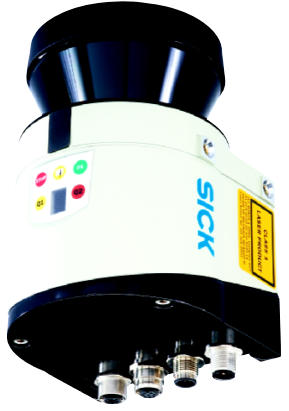
\includegraphics[width=0.16\linewidth]{img/chap_lidar/lms151.png}}
    \subfloat[]{\label{fig:lidar_basics_b}}{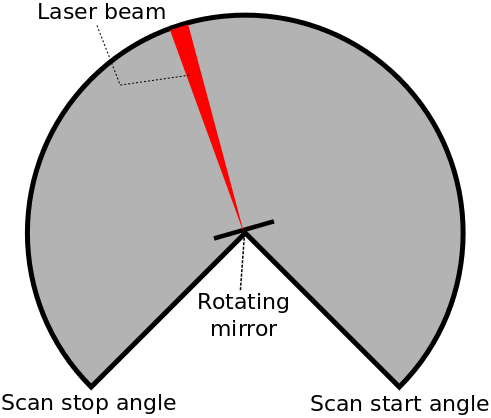
\includegraphics[width=0.28\linewidth]{img/chap_lidar/lidar_mirror.png}}
    \subfloat[]{\label{fig:lidar_basics_c}}{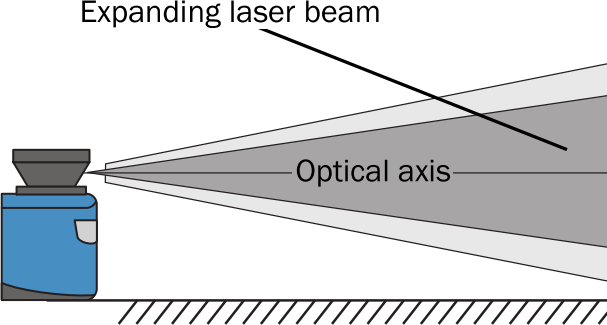
\includegraphics[width=0.44\linewidth]{img/chap_lidar/sick_beam_adapted.png}}
    \caption[Example of a \gls*{lidar} device and a simplified representation of the laser trajectory.]{Example of a \gls*{lidar} device and a simplified representation of the laser trajectory. \protect\subref{fig:lidar_basics_a} The SICK LMS151 \gls*{lidar}. The truncated cone of the upper part is the place from where the laser is projected and is made of a material allowing the laser to pass through unaffected. \protect\subref{fig:lidar_basics_b} A simplified representation of how the internal rotating mirror change the scanning angle of the laser. \protect\subref{fig:lidar_basics_c} A side view of the laser beam going out of the \gls*{lidar} (figure modified from~\citep{LMS151Manual}).}
    \label{fig:lidar_basics}
\end{figure}

Beams emitted by a \gls*{lidar} have a given with width and angle at source. This cause the beam two-dimensional pattern on the target to grow with distance. Once the light hit the target, it bounces back to the sensor which will extract the range information out of it. Obviously, when the target material is highly absorbent or reflective, the light might not reach back the sensor, therefore causing missing data points. Otherwise, the sensor will receive the signal which may be represented by a curve of light intensity as function of time. Smooth lambertian surfaces will produce a unimodal distribution with which it is easy to calculate the target range, but multi-modal waveforms caused by partially transparent material, fog, dust, small objects and edges lead to an ambiguous interpretation. Figure~\ref{fig:lidar_waveform} depict laser beam hitting different targets along with the resulting waveforms. While some \gls*{lidar}s provide full waveform, they generally only output a single or few echoes and the inference method differs from sensor to sensor (e.g., using the first or last waveform peak, using the mean). For this reason, it is important to determine whether the sensor of your choice is well suited to your needs. 

In order to visualize more easily the data obtained with a lidar, they are typically represented by a point cloud. Building such point cloud only consist in converting each distance inferred from a laser return into a point in the \gls*{3d} space. Figure~\ref{fig:shadow_points} show an example of a scene \subref{fig:shadow_points_a} and the corresponding point cloud representation \subref{fig:shadow_points_b}. There are also highlighted regions of the point cloud where you can see examples of reading errors caused by the environment surrounding the robot. 

In this document, we focus our attention on the impact of small structures such as the branch presented in Figure~\ref{fig:shadow_points_b} region \textbf{D}. More specifically, the present chapter deal with the impact of falling snow on the raw data of \gls*{lidar}s. In the next section (Section~\ref{sec:chap_lidar_data_acquisition}), we will explain how we gathered data for this analysis.

\begin{figure}[h]
    \centering
    \subfloat[]{\label{fig:lidar_waveform_a}}{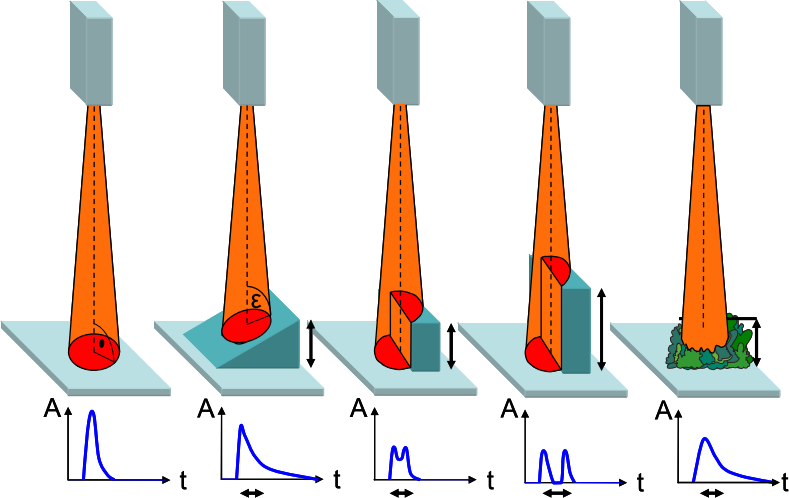
\includegraphics[width=0.8\linewidth]{img/chap_lidar/waveforms.png}}\\\vspace{1em}
    \subfloat[]{\label{fig:lidar_waveform_b}}{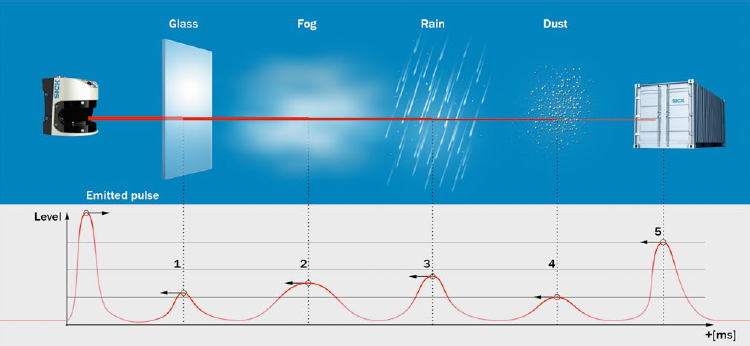
\includegraphics[width=0.8\linewidth]{img/chap_lidar/waveforms2.png}}
    \caption[Representation of \gls*{lidar} beams in different conditions along with the resulting waveforms.]{Representation of \gls*{lidar} beams in different conditions along with the resulting waveforms. \protect\subref{fig:lidar_waveform_a} Differents unimodal and multimodal distribution resulting from different target structures. From \citet{lidar_figure1}. \protect\subref{fig:lidar_waveform_b} The multimodal waveform resulting from a laser beam going through multiple translucent material. From the SICK LMS500-21000 Lite website~\citep{sick_waveform}.}
    \label{fig:lidar_waveform}
\end{figure}

\begin{figure}[h]
    \centering
    \subfloat[]{\label{fig:shadow_points_a}}{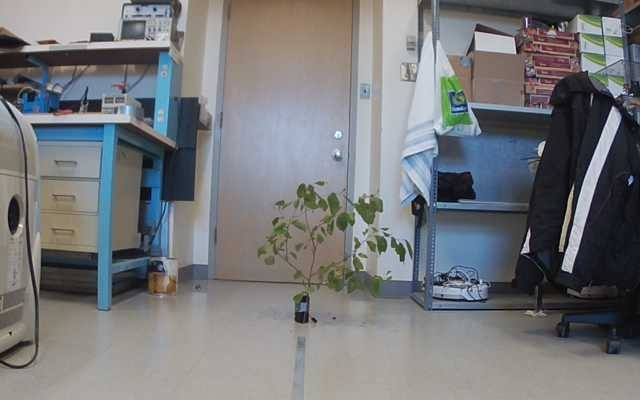
\includegraphics[width=0.9\linewidth]{img/chap_lidar/shadow_image.jpg}}\\\vspace{1em}
    \subfloat[]{\label{fig:shadow_points_b}}{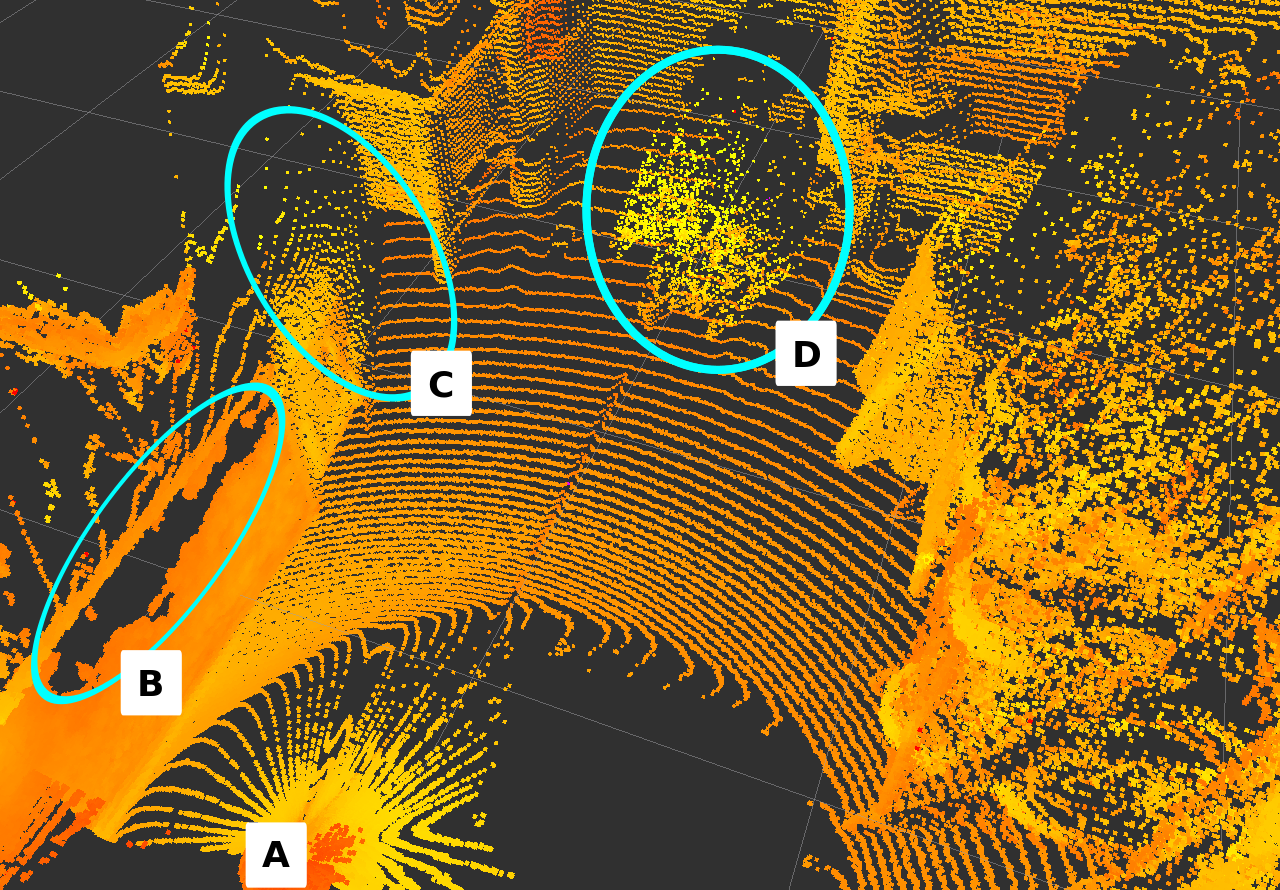
\includegraphics[width=0.9\linewidth]{img/chap_lidar/shadow_pointcloud.png}}
    \caption[Point cloud representation of a \gls*{lidar} acquisition and examples of erroneous data regions.]{A picture of a scene \protect\subref{fig:shadow_points_a} and a diagonal view of the point cloud \protect\subref{fig:shadow_points_b} resulting from the acquisition by the SICK LMS151 \gls*{lidar} mounted on a \gls*{ptu}. The sensor position is represented by \textbf{A}. Region \textbf{B} shows missing points caused by absorbent material (a black box not visible in the picture). Region \textbf{C} shows noisy points caused by the edge of an object while region \textbf{D} shows a particularly bad \gls*{3d} representation of a fine structure (tree branch).}
    \label{fig:shadow_points}
\end{figure}
